\noindent
\begin{tabular}{cc}
\begin{minipage}[b]{0.65\textwidth}
\begin{exerciseS}[Capillare]
Sia $\theta$ l'angolo di contatto all'interfaccia tra aria, liquido e solido; 
sia $\gamma$ la tensione superficiale tra aria e liquido; sia $\rho$ la densità del liquido.
Determinare l'altezza $h$ dal liquido in una colonnina cilindrica di raggio $r = 0.5 \ mm$  rispetto al livello
nella vasca. Calcolare poi la pressione all'interno della colonnina.
(Si può considerare valida l'approssimazione che la pressione agente sulla vasca e sulla superficie
superiore del liquido all'interno della colonnina sia uguale).

\vspace{0.1cm}
Si considerino condizioni termodinamiche e materiale della colonnina tali che:
se il liquido è acqua: $\rho = 999 \ kg/m^3$, $\theta={1}\degree$, $\gamma=0.073 N/m$.
se il liquido è mercurio: $\rho = 13579 \ kg/m^3$, $\theta={140}\degree$, $\gamma=0.559 N/m$.
($h_{H_2O} = 2.97 \ cm$, $P_{H_20} - P_0 =  - 291.95 \ Pa$; $h_{Hg} = -1.28 \ cm$, $P_{Hg} - P_0 =  1712.87 \ Pa$)
\end{exerciseS}
\end{minipage}
&
\begin{minipage}[b]{0.35\textwidth}
   \begin{center}
   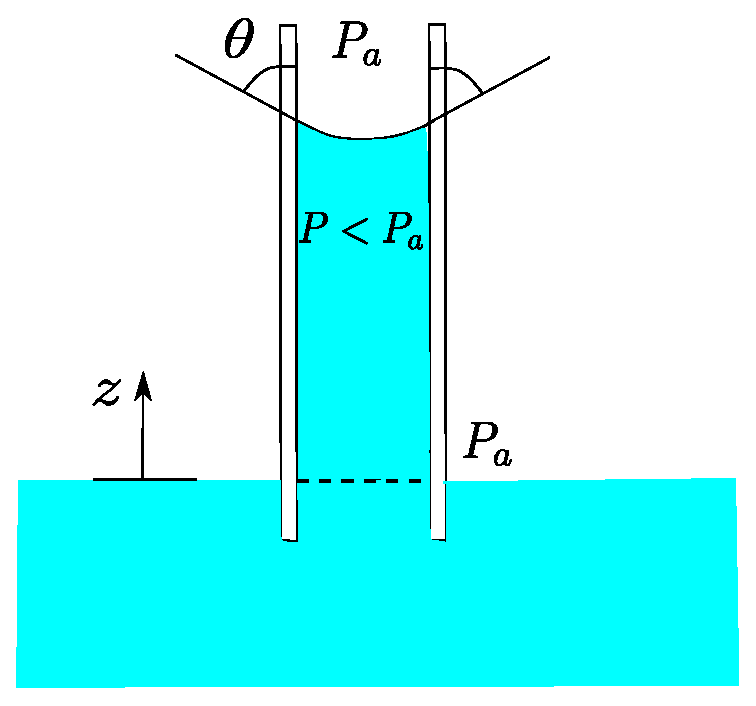
\includegraphics[width=0.80\textwidth]{./fig/cap01.eps}
   \end{center}
\end{minipage}
\end{tabular}

\sol

\partone
 Tensione superficiale. Angolo di contatto. Capillarità. Menisco.

\parttwo
 Scrivendo l'equilibrio per il volume di fluido nel capillare si trova l'altezza $h$.
Successivamente si trova la $p$ usando la legge di Stevino. Infine si fanno osservazioni su angolo di contatto,
menisco e salto di pressione all'interfaccia.
%
\begin{itemize}
\item Si scrive l'equilibrio del volume di fluido. Il problema è di statica. Le forze agenti sono la forza
dovuta alla tensione superficiale (che agisce sul perimetro della superficie superiore) e la forza peso, poichè per ipotesi la pressione agente sulla superficie superiore è uguale alla pressione ambiente $P_a$; e quindi??? Perchè la componente verticale della risultante dovuta alla pressione esterna è zero??? Vedere immagine...).
%
\begin{equation}
  F_{\gamma} = F_g \quad \Rightarrow \quad 2\pi r \gamma  \cos \theta = \pi r^2 h \rho g
\end{equation}
%
E quindi: 
\begin{equation}
  h = \frac{2 \gamma \cos \theta}{\rho g r}
  \quad \Rightarrow \quad
  \begin{cases}
    h_{H_20} = 2.97 \ cm \\
    h_{Hg} = -1.28 \ cm
  \end{cases}
\end{equation}
%
\textit{Commenti sul risultato.} L'effetto della capillarità è più evidente per tubi stretti (proporzionalità con $1/r$). La quota $h$ può assumere sia valori positivi, sia valori negativi, 
in base al valore dell'angolo di contatto: $h \le 0$, per $\theta \ge \pi/2$.
%
%\begin{figure}[h]
%\centering
%\captionsetup[subfigure]{labelformat=empty}
%\subfloat[][\emph Equilibrio del volume di fluido nella colonnina. La pressione atmosferica $P_a$ non
%   influenza l'equilibrio. Perchè?]
%   {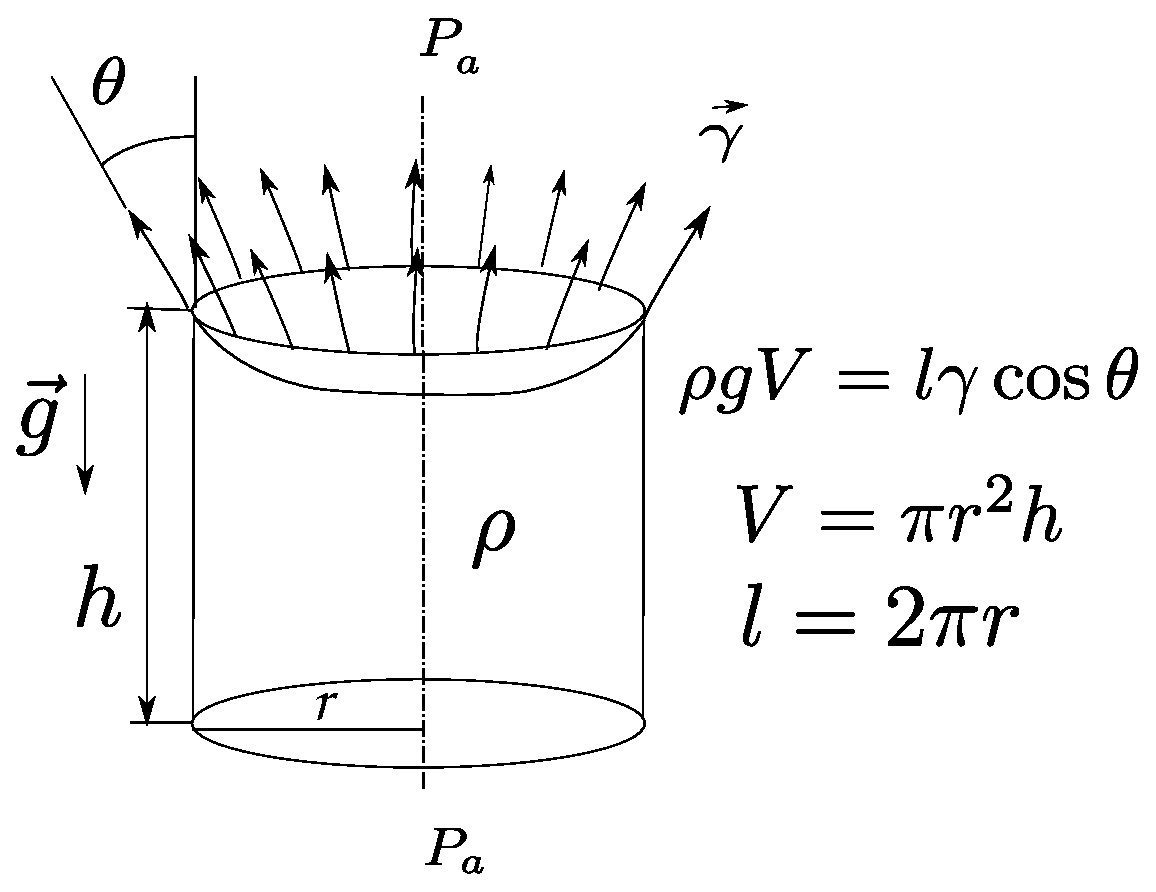
\includegraphics[width=0.30\textwidth]{./fig/equil.eps}}
%\end{figure}
%
\item Si calcola la pressione nel fluido in cima alla colonnina sfruttando la legge di Stevino.
\begin{equation}
  P = P_0 - \rho g h = P_0 - \frac{2 \gamma \cos \theta}{r}
  \quad \Rightarrow \quad
  \begin{cases}
    P_{H_20} - P_0 =  - 291.95 \ Pa \\
    P_{Hg}   - P_0 =  1712.87 \ Pa
  \end{cases}
\end{equation}
%
\textit{Commenti sul risultato.}  $P-P_0 \le 0$, per $\theta \le \pi/2$. Al contrario $P-P_0 \ge 0$, per $\theta \ge \pi/2$. Questi risultati sono compatibili (meno male) con le relazioni tra curvatura (stretta parente del menisco e dell'angolo di contatto) e il salto di pressione.
%
\begin{center}
  \begin{tabular}{ c c c }
    \hline
    $\theta \le \pi/2$ & $h \ge 0$  & $P \le P_a$ \\ \hline
    $\theta \ge \pi/2$ & $h \le 0$  & $P \ge P_a$ \\ \hline
  \end{tabular}
\end{center}

\begin{figure}
\centering
%\captionsetup[subfigure]{labelformat=empty}
\subfloat[][\emph Differenza tra il menisco formato dall'acqua e dal mercurio 
    con aria e solido (quale?): diversa concavità della superficie. ]
   {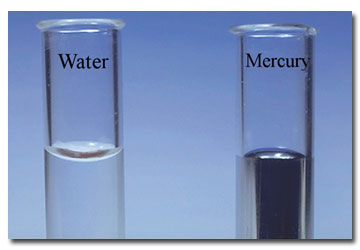
\includegraphics[width=0.32\textwidth]{./fig/menisco.jpg}} \quad
\subfloat[][\emph Rappresentazione del caso del problema in cui il liquido è mercurio: 
    l'angolo di contatto è maggiore dell'angolo retto, la quota all'interno del capillare
    è minore di quella nella vasca. Il caso dell'acqua è rappresentato a finaco del testo del problema.]
   {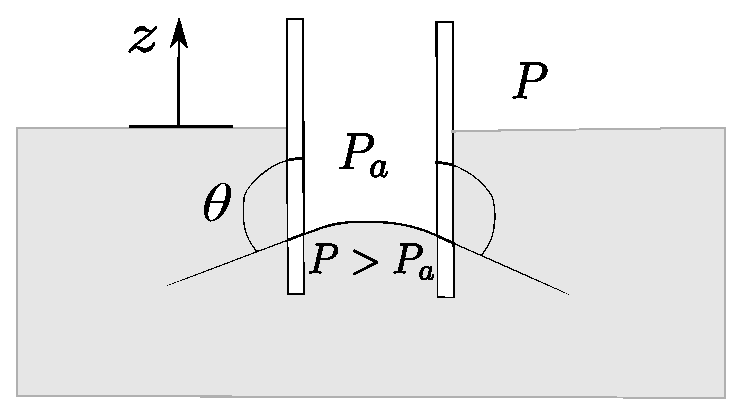
\includegraphics[width=0.32\textwidth]{./fig/cap02.eps}} \quad
%\subfloat[][\emph Rappresentazione delle condizioni all'interfaccia tra due fluidi quando viene considerato il contributo della tensione superficiale: secondo la formula di Young-Laplace vale $\bm{t_A} - \bm{t_B} = \gamma \bm{\hat{n}} (\frac{1}{R_1} + \frac{1}{R_2})$, dove $\bm{\hat{n}}$ è la normale e $R_1$, $R_2$ sono i raggi di curvatura della superficie. ]
%   {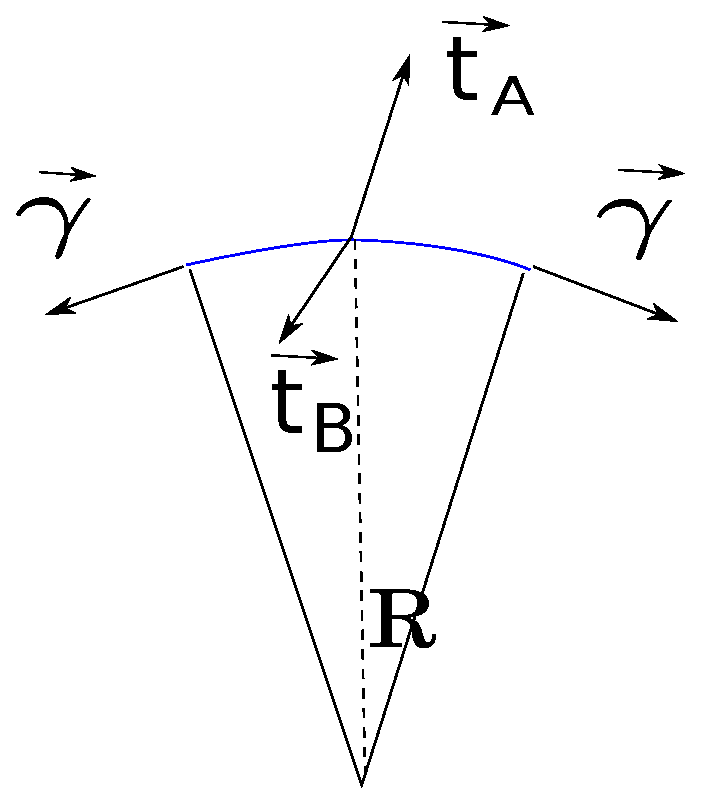
\includegraphics[width=0.22\textwidth]{./fig/laplaceYoung2D.eps}}
\subfloat[][\emph Equilibrio del volume di fluido nella colonnina. La pressione atmosferica $P_a$ non
   influenza l'equilibrio. Perchè?]
   {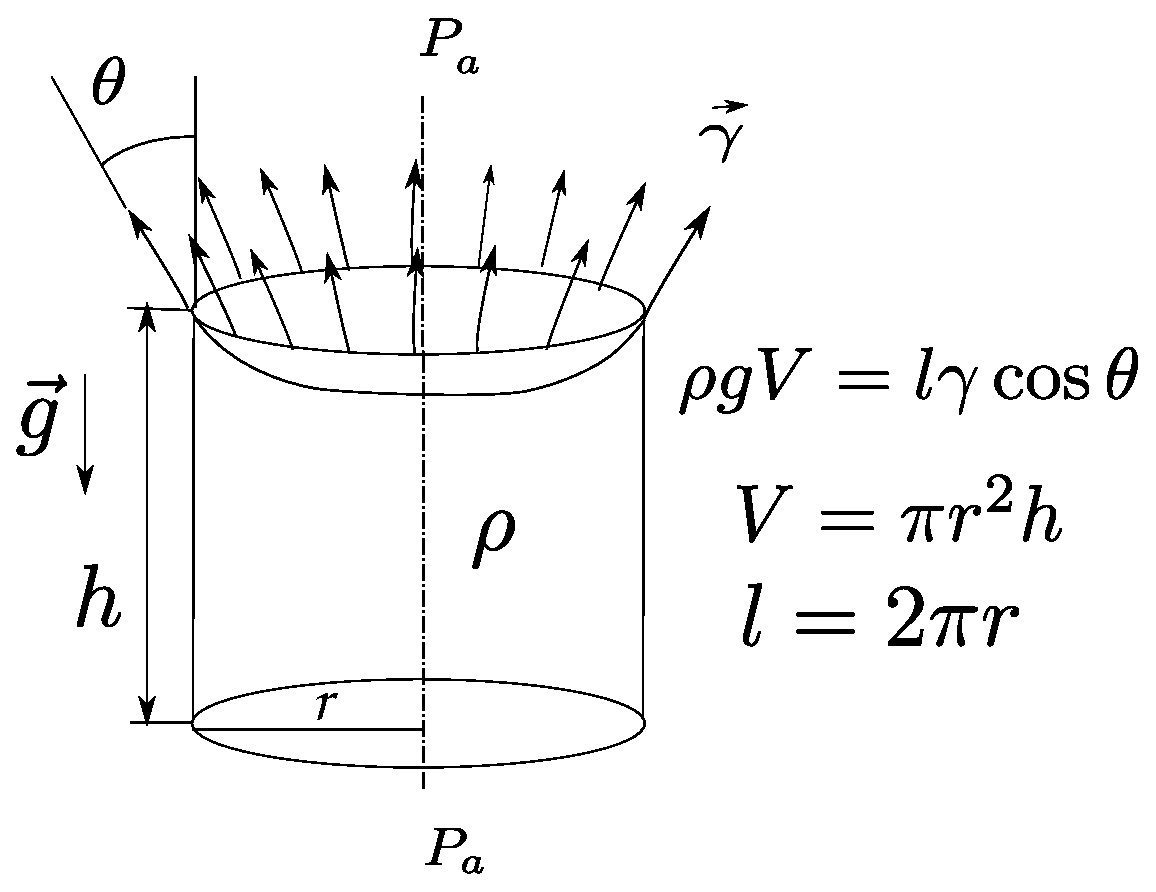
\includegraphics[width=0.30\textwidth]{./fig/equil.eps}}
\end{figure}


\end{itemize}










